\documentclass[fullscreen=true, unicode, bookmarks=false]{beamer}

\usepackage{lmodern}

\usepackage[T2A]{fontenc} 
\usepackage[cp1251]{inputenc}
\usepackage[russian]{babel}
\usepackage{amsmath,amsfonts,amssymb}
\usepackage[export]{adjustbox}
\usepackage{textgreek}
\sloppy

\setbeamertemplate{navigation symbols}{}

\usetheme{Madrid}

\usecolortheme{whale}

\usefonttheme{professionalfonts} % default family is serif

\setbeamertemplate{footline}{\hspace*{.5cm}\scriptsize{\insertshorttitle
\hspace*{50pt} \hfill\hspace*{.5cm}}\vspace{5pt}} 

\setbeamercolor{bibliography entry author}{fg=black}

\title[]{ Oscillating loss of stability of trivial solution for boundary-value problem with linear deviate in boundary condition }   
\author[]{{\large Leonid Ivanovsky, Ilya Kuksenok}} 
\date{}
\institute[]
{ postgraduate students }
\titlegraphic{
   \vspace{-0.5cm}
   
\includegraphics[scale = 0.5]{yarsu_logo.png}
   \hspace{2cm}
   
\includegraphics[scale = 0.9]{mephi_logo.png}
}

\begin{document}

\begin{frame}
\titlepage
\end{frame} 

\begin{frame}
\frametitle{ Nonlinear boundary-value problem }
 
\begin{equation}\label{ivanovsky-eq1}
	u' = \beta \ddot{u} - \gamma u(t - \tau) + F(u),
\end{equation}	

\begin{gather}\label{ivanovsky-eq2}	
	u'(0, t) \, = 0, \\
	u'(1, t) \, = \alpha\,u(x_0, t-\tau). \nonumber
\end{gather}

$$ \alpha \in \mathbb{R}, \quad \beta, \gamma > 0, \quad \tau \geqslant 0, \quad x_0 \in [0, 1]. $$

\medskip
\pause

\begin{exampleblock}{}
{\large Kaschenko S.A. About bifurcations with small disturbances in logistic equation with delay // Modelling and Analysis of Information Systems, v.24(2), p. 168--185 (2017). }
\end{exampleblock}

\end{frame}

\begin{frame}
\frametitle{ Nonlinear boundary-value problem without delay}
 
\begin{equation}\label{ivanovsky-eq3}
	u' = \beta \ddot{u} - \gamma u + F(u),
\end{equation}	

\begin{gather}\label{ivanovsky-eq4}	
	u'\mid_{x=0} \, = 0, \\
	u'\mid_{x=1} \, = \alpha\,u\mid_{x=x_0}. \nonumber
\end{gather}

$$ \alpha \in \mathbb{R}, \quad \beta, \gamma > 0, \quad x_0 \in [0, 1]. $$

\medskip

\begin{exampleblock}{}
{\large This work is supported by the Russian Science Foundation (project nos. 14-21-00158). }
\end{exampleblock}

\end{frame}

\begin{frame}
\frametitle{ Substitutions }
	
$$ t_1 = d \times t, $$

\bigskip

$$ u(x, t) = w(x)\,\mbox{exp}\left( \lambda - \frac{\gamma}{d}t \right). $$

\end{frame}


\begin{frame}
\frametitle{ Simplified boundary-value problem }
	
\begin{equation}\label{ivanovsky-eq5}
	w'' - \lambda w = 0,
\end{equation}

\begin{gather}\label{ivanovsky-eq6}	
	w'(0) = 0, \\
	w'(1) = \alpha\,w(x_0). \nonumber
\end{gather}

\end{frame}

\begin{frame}
\frametitle{ Boundary conditions }

$$ w(x) = c \, \mbox{ch} (\mu\,x), $$

$$ \mu^2 = \lambda. $$

\vspace{1.1cm}
\pause
	
$$ x = 1: $$

$$ \mu \sh \mu = \alpha \ch(\mu x_0). $$

\end{frame}

\begin{frame}
\frametitle{ System of equations }
	
$$ \lambda \in \mathbb{C}: \quad \mu = \tau + i \omega. $$

\bigskip

\begin{equation}\label{ivanovsky-eq7}
\begin{array}{l}
\begin{cases}
f(\tau, \omega) = 0 \\
g(\tau, \omega) - \alpha = 0. \\
\end{cases}
\end{array}
\end{equation}

\end{frame}

\begin{frame}
\frametitle{ Oscillating loss of stability of zero balance state }
	
\begin{theorem}
There exists $ \alpha=\alpha_{cr} $, for that $ \mbox{Re}(\lambda_{*}) = \dfrac{\gamma}{\beta} $ and for the rest eigenvalues of problem (3), (4) $ \mbox{Re}(\lambda) < \dfrac{\gamma}{\beta} $ 
\end{theorem}

\vspace{1.1cm}
\pause

\begin{exampleblock}{}
{\large Ivanovsky L.I., Kaschenko S.A. Stability loss of the trivial solution of boundary-value problem with linear deviate in boundary conditions // International Scientific Conference "New trends in nonlinear dynamics". Abstracts, p. 32-33 (2017). }
\end{exampleblock}
\end{frame}

\begin{frame}
\frametitle{ Numerical research } 

\begin{figure} 

\includegraphics[scale=0.25]{python.png}  
\hfill

\includegraphics[scale=0.6]{openmp.jpg} 
\end{figure}

\end{frame}

\begin{frame}
\frametitle{ Algorithm } 

\begin{figure} 
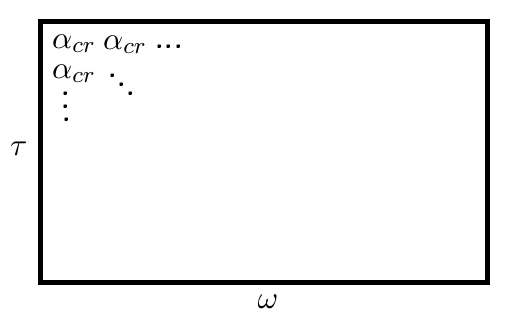
\includegraphics[scale=0.45]{algo.png}  
\end{figure}

$$ \omega \rightarrow \tau_{*} \rightarrow \alpha_{*} $$

$$ \mbox{Re}(\lambda_{*}) = \frac{\gamma}{\beta} = \tau_{*}^2 - \omega^2 $$ 

\end{frame}

\begin{frame}
\frametitle{ Algorithm } 

$$ \alpha = \alpha_{cr}: \quad |\alpha_{*}-\alpha| < \varepsilon $$

\pause

\begin{gather*}	
	\alpha_{*} = \tau_{*}^2 - \omega^2 \\
	\alpha = \tau^2 - \omega^2 \nonumber
\end{gather*}

\pause

$$ \mbox{Re}(\lambda) < \mbox{Re}(\lambda_{*}) + \varepsilon $$

\end{frame}

\begin{frame}
\frametitle{Results} 
\begin{figure}[h]
\begin{minipage}[h]{0.49\linewidth}
\center{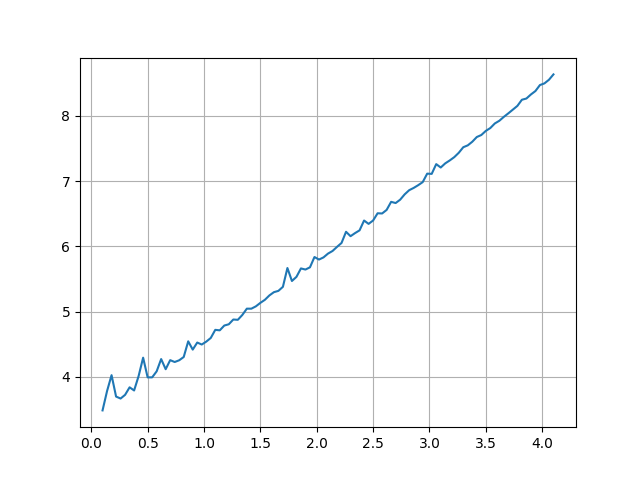
\includegraphics[scale=0.27]{0,0.png} \\ {\tiny $ x_0 = 0.0 $}}
\end{minipage}
\hfill
\begin{minipage}[h]{0.49\linewidth}
\center{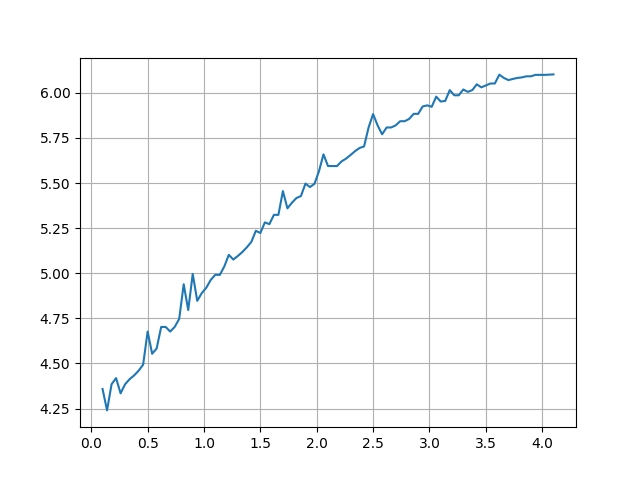
\includegraphics[scale=0.27]{0,15.png} \\ {\tiny $ x_0 = 0.15 $}}
\end{minipage}
\vfill
\begin{minipage}[h]{0.49\linewidth}
\center{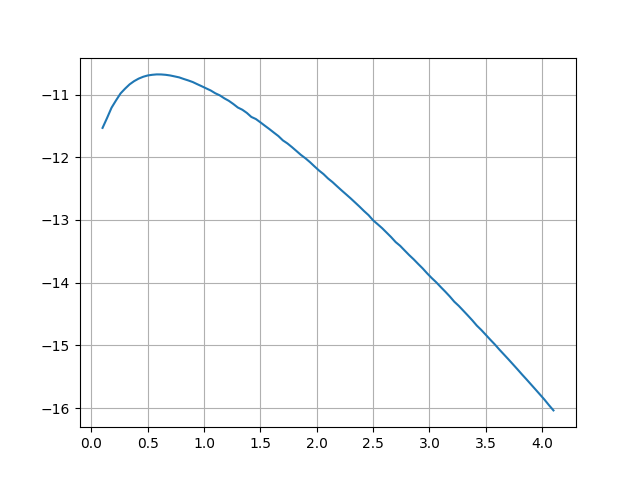
\includegraphics[scale=0.27]{0,45.png} \\ {\tiny $ x_0 = 0.45 $}}
\end{minipage}
\hfill
\begin{minipage}[h]{0.49\linewidth}
\center{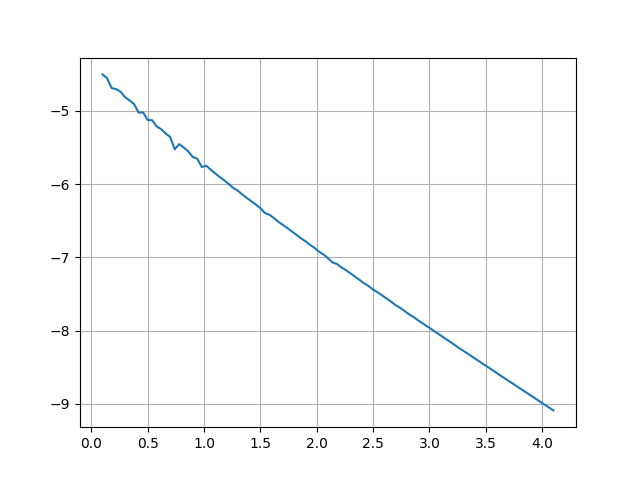
\includegraphics[scale=0.27]{0,6.png} \\ {\tiny $ x_0 = 0.6 $}}
\end{minipage}
\center{ {\scriptsize $ \beta = 1.0 $} }
\end{figure}
\end{frame}

\begin{frame}
\frametitle{ Nonlinear boundary-value problem with delay}
 
\begin{equation}\label{ivanovsky-eq8}
	u' = \beta \ddot{u} - \gamma u(t - \xi) + F(u),
\end{equation}	

\begin{gather}\label{ivanovsky-eq9}	
	u'\mid_{x=0} \, = 0, \\
	u'\mid_{x=1} \, = \alpha\,u(1, t-\tau). \nonumber
\end{gather}

$$ \alpha \in \mathbb{R}, \quad \beta, \gamma > 0, \quad \tau,\xi> 0. $$

\end{frame}
\begin{frame}
\frametitle{Linear problem}
\begin{equation}
	u' = \beta \ddot{u} - \gamma u(t - \xi)
\end{equation}
\begin{equation}
	u(x,t) = X(x) \exp(\lambda t)
\end{equation}
\begin{equation}\label{kuksenok-eq1}
(\ref{ivanovsky-eq8}, \ref{ivanovsky-eq9}) \quad \rightarrow \quad
\left\{
\begin{matrix}
    \ddot{X}-\frac{1}{\beta}\left( \lambda + \gamma  \exp(-\lambda \xi) \right) X = 0\\
    \dot{X}|_{x=0}=0\\
    \dot{X} - \alpha \exp{(-\lambda \tau)} X |_{x=1} = 0
\end{matrix}
\right.
\end{equation}
\end{frame}
\begin{frame}
\frametitle{Quasi analytic solution}
Let 
\begin{equation}\label{kuksenok-eq2}
g = \frac{1}{\beta}\left( \lambda + \gamma  \exp(-\lambda \xi) \right),
\end{equation}
so
\begin{equation}\label{kuksenok-eq3}
(\ref{kuksenok-eq1}, \ref{kuksenok-eq2}) \quad \rightarrow \quad
\left\{
\begin{matrix}
    g^{1/2}\sh{g^{1/2}}-\alpha \exp{(-\lambda \tau)} \ch{g^{1/2}} = 0 & \mbox{if } \tau \neq 0 \\
    g^{1/2}\sh{g^{1/2}}-\alpha \, \alert{1} \, \ch{g^{1/2}} = 0 & \mbox{if } \tau = 0
\end{matrix}
\right.
\end{equation}
\end{frame}
\begin{frame}
\frametitle{Quasi analytic solution}
Let's solve (\ref{kuksenok-eq2})
\begin{equation}\label{kuksenok-eq4}
\lambda \, = \, \frac{\alert{g} \beta \xi - \text{W}(k,-\exp{(-\alert{g} \beta \xi) \gamma \xi})}{\xi},
\end{equation}
where $g$ can be found as a numerical solution of (\ref{kuksenok-eq3})
\end{frame}
\begin{frame}
Roots of (\ref{kuksenok-eq3}) can be found numerically for different $\alpha $
\begin{center}$
\begin{aligned}
&\alpha = 0.5 \quad g \rightarrow  0.59552; \\
&\alpha = 1.0 \quad g \rightarrow 1.43923; \\
&\alpha = 1.5 \quad g \rightarrow  2.63030; \end{aligned}$ 
\end{center}
\end{frame}

\begin{frame}
\frametitle{ $\alpha = 0.5 \quad g \rightarrow  0.59552$ }
\center{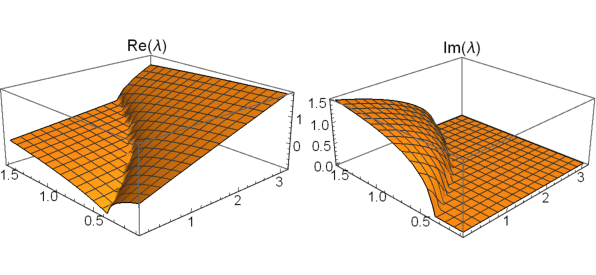
\includegraphics[scale=1]{al05.pdf} \\ {\tiny $ k = 0, \tau =0, \xi = 1$} \\ $\beta_{crit} \rightarrow 0.93612 \quad \gamma_{crit} \rightarrow 1.23716$ \\ $\alert{Im(\lambda_{crit})\rightarrow1.10347}$ \\  $Re(\lambda_{crit}) << 10^{-6}$ }  
\end{frame}
\begin{frame}
\frametitle{ $\alpha = 1.0 \quad g \rightarrow 1.43923$ }
\center{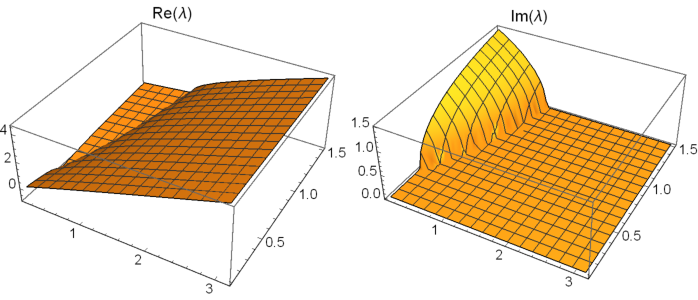
\includegraphics[scale=1]{al10.pdf} \\ {\tiny $ k = 0, \tau =0, \xi = 1$} \\ $\beta_{crit} \rightarrow 0.33334 \quad \gamma_{crit} \rightarrow 1.28224$ \\ $\alert{Im(\lambda_{crit})\rightarrow 1.18855}$ \\  $Re(\lambda_{crit}) << 10^{-6}$ }
\end{frame}
\begin{frame}
\frametitle{ $\alpha = 1.5 \quad g \rightarrow 2.63030$ }
\center{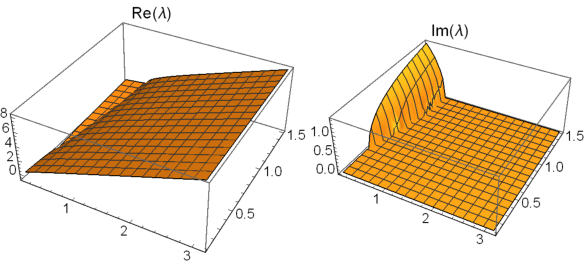
\includegraphics[scale=1]{al15.pdf} \\ {\tiny $ k = 0, \tau =0, \xi = 1$} \\ $\beta_{crit} \rightarrow 0.18224 \quad \gamma_{crit} \rightarrow 1.28323$ \\ $\alert{Im(\lambda_{crit})\rightarrow 1.19032}$ \\  $Re(\lambda_{crit}) << 10^{-6}$ }
\end{frame}

\begin{frame}
\frametitle{ LambertW }
\begin{flushleft}
    \begin{enumerate}
        \item $f(W)=W\exp{(W)}$
        \item $\text{W}(-\frac{1}{e})=-1$
        \item $\text{W}(e)=1$
        \item $\frac{\text{W}(z)}{d z}=\frac{1}{1+\exp{(\text{W}(z))}}$
    \end{enumerate}
\end{flushleft}
\begin{flushright}
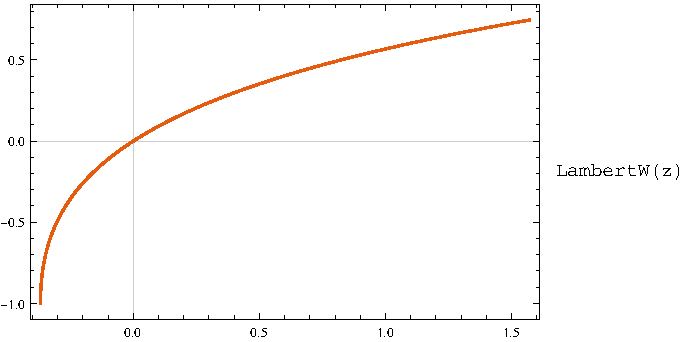
\includegraphics[scale=0.7]{W_z.pdf}
\end{flushright}
\end{frame}
\end{document}